	\chapter{Testf"alle und Resultate}
	In diesem Abschnitt sollen die Ergebnisse und die Effizienz des in Abschnitt \ref{cha:program_description} vorgestellten Programmes anhand von zwei unterschiedlichen Testf"allen analysiert werden. Als Referenz dient dabei das Programm \texttt{MC3D} \citep{Wolf:2003p12974}, sowohl f"ur die berechneten Bilder als auch f"ur die Geschwindigkeit der Berechnung. F"ur den ersten Testfall wurde zur Berechnung einer Referenzl"osung zus"atzlich zum einen ein geschlossener Ausdruck f"ur die L"osung hergeleitet und zum anderen ein einfaches Monte--Carlo--Verfahren erdacht, das sehr schnell konvergiert.
	
	\section{Homogene streuende Kugel}
	Um die Korrektheit der vom Monte--Carlo--Code produzierten L"osung zu verifizieren ist es von erheblichem Nutzen eine unabh"angig gewonnene, vielleicht sogar analytisch hergeleitete, L"osung eines konstruierten Testproblems berechnen zu k"onnen. Das Problem sollte dabei nicht so trivial sein, da"s komplexe Effekte wie Mehrfachstreuung keinen Einflu"s auf das Ergebnis haben. Gleichzeitig sollte es aber nicht so komplex sein, da"s keine elegante, leicht berechenbare L"osung gefunden werden kann.
	Mit dieser Motivation konstruieren wir folgendes Testproblem:
		
	Gegeben sei eine Kugel mit Radius $R$, die mit homogenem, isotrop streuendem Material mit Volumenstreuquerschnitt $\sigma=1$ gef"ullt ist, sowie eine punktf"ormige Lichtquelle im Zentrum der Kugel. Zu berechnen ist nun die radiale Abh"angigkeit der Intensit"at, die eine ausserhalb der Kugel platzierte orthographische Kamera, die zum Zentrum der Kugel ausgerichtet ist, misst. Die feste Wahl von $\sigma$ und Variation des Kugelradius $R$ dient ausschliesslich der einfacheren Berechnung, da die Wegstrecken dadurch automatisch in optischen Wegl"angen $\lambda=1/\sigma$ vorliegen. Das Problem ist gleichwertig zu jeder anderen Kombination aus Radius und Volumenstreuquerschnitt f"ur welche sich die gleiche optische Tiefe $\tau_\text{center}=\sigma R=R/\lambda$ vom Zentrum bis zum Rand der Kugel ergibt.
	
	\begin{figure}
			\centering
			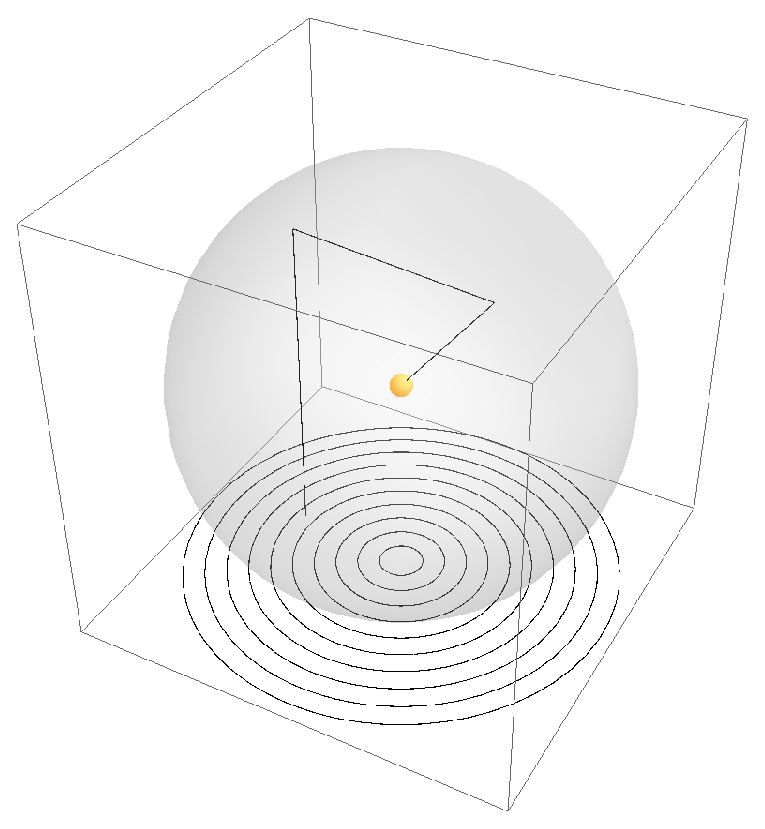
\includegraphics[width=0.6\textwidth]{testproblem_illustration.eps}
			\caption{Illustration des Testproblems. Gezeigt ist ein Photonenpfad der zweimal gestreut wird und in einem ringf"ormigen Bin der orthographischen Kamera auftrifft}
			\label{fig:testproblem_sketch}
	\end{figure}

	
	\subsection{analytische L"osung}\label{subsec:homsphere_analytic_solution}
	\subsubsection{Green'sche Funktion f"ur den Photonentransport zwischen Kugelschalen}
	Um die korrekte radiale Intensit"atsverteilung zu berechnen, bestimmen wir zun"achst in Form der Green'schen Funktion $g$, wie sich die Photonen radial nach einem Streuvorgang ausgebreitet haben.
	Genauer gibt $g$ an, wie gro"s der Anteil der Photonen, die auf einer Kugelschale mit Radius $r_0$ starten, beim Radius $r_1$ w"ahrend des n"achsten Streuvorganges ist (siehe Abb. \ref{fig:radial_greens_function_pdfcdf}):
	\begin{align*}
		g(r_0,r_1) =& 2 \pi \int_0^\pi r_1^2 \sin \theta \frac{\exp\left(-\sqrt{r_0^2-2 r_0 r_1 \cos(\theta)+r_1^2}\right)}{4 \pi (r_0^2-2 r_0 r_1 \cos(\theta)+r_1^2)} \text{d}\theta \\
		=& \frac{1}{2}\frac{r_1}{r_0} \int_{|r_0-r_1|}^{r_0+r_1} \frac{e^{-t}}{t} dt \\
		=& \frac{1}{2}\frac{r_1}{r_0}\left[\text{Ei}(-(r_0+r_1)) - \text{Ei}(-|r_0-r_1|)\right]
	\end{align*}
	
	\begin{figure}
		\centering
		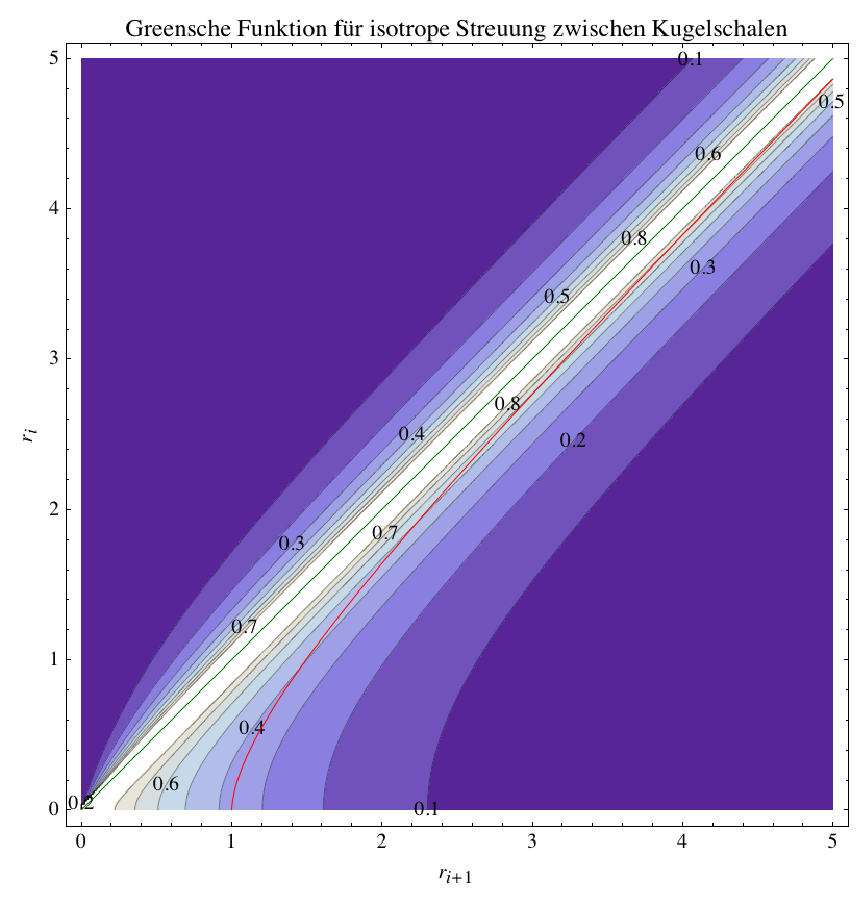
\includegraphics[width=0.48\textwidth]{radial_greens_function_pdf.eps}
		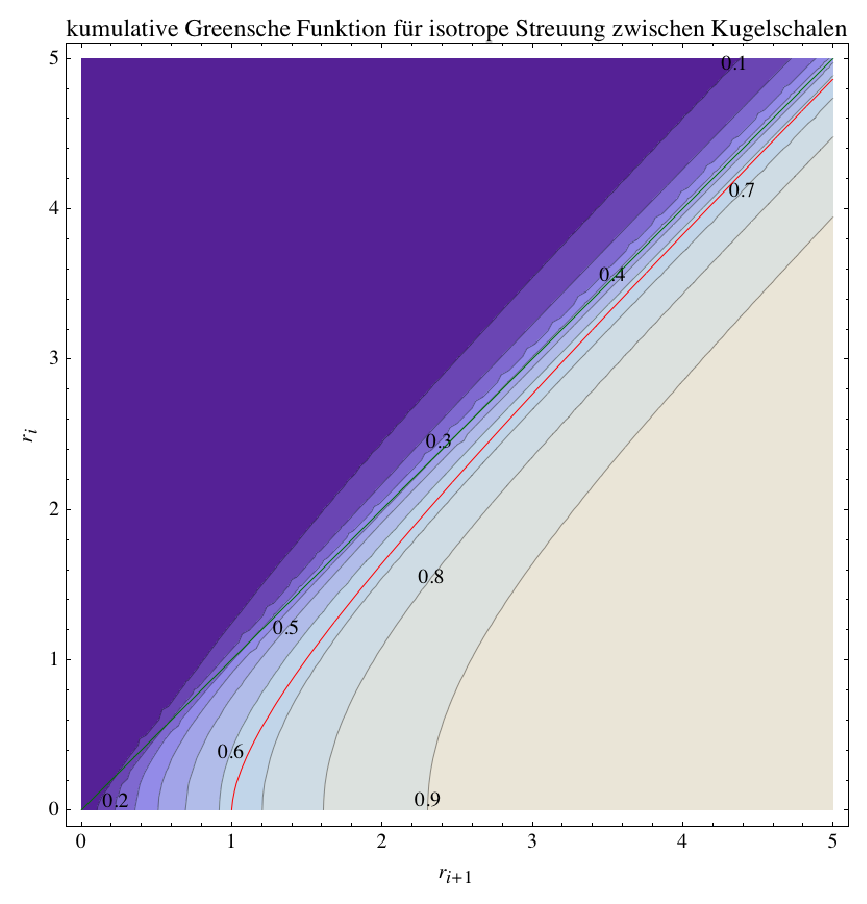
\includegraphics[width=0.48\textwidth]{radial_greens_function_cdf.eps}
		\caption{Green'sche Funktion der radialen Teilchenverteilung die von Radius $r_i$ kommen und beim Radius $r_{i+1}$ streuen als PDF und CDF. Der mittlere Radius ist in rot eingezeichnet.}
		\label{fig:radial_greens_function_pdfcdf}
	\end{figure}
	\begin{figure}
		\centering
		\includegraphics[width=0.9\textwidth]{gnlist_plot.eps}
		\caption{radiale Photonenverteilung nach n Streuvorg"angen. Die freie optische Wegl"ange ist dabei mit $\lambda=1/\sigma$ bezeichnet.}
		\label{fig:gnlist}
	\end{figure}
	Als n"achstes diskretisieren wir die Green'sche Funktion, indem wir ein gleichm"assiges Gitter in $r_0$ und $r_1$ "uber $g$ legen, das sich bis zum Radius der Kugel $R$ erstreckt, und innerhalb jeder Gitterzelle $g$ in $r_0$--Richtung mitteln und in $r_1$--Richtung aufintegrieren und anschliessend die Ergebnisse in einer Matrix $\mathbf{g}$ speichern. Wenn wir nun einen Startvektor, der nur in der innersten Zelle von Null verschieden ist, $n$--mal mit $\mathbf{g}$ multiplizieren, bekommen wir die diskretisierte Photonenverteilung innerhalb der Kugelschalen beim $n$--ten Streuvorgang (siehe Abb. \ref{fig:gnlist}). Um die Emissivit"at $\varepsilon(r)$ jeder Kugelschale auszurechnen, summieren wir die Photonenverteilungen vom 1--ten bis zum $n$--ten Streuvorgang auf und teilen das Ergebnis in jeder Kugelschale durch ihr jeweiliges Volumen und den bestrahlten Raumwinkel $4\pi$. Die Intensit"aten berechnen wir nun numerisch gem"a"s
	\begin{equation}
		I(r) = \int_{z=-h}^h \varepsilon\left(\sqrt{r^2+z^2}\right) e^{-(z+h)}\text{d}z\,,\quad h=\sqrt{R^2-r^2}
		\label{eq:testprob_intensity_calculation}
	\end{equation}
	
	%\begin{figure}
	%	\centering
	%	\includegraphics[width=1.0\textwidth]{analytical_tau_comparison.eps}
	%	\caption{radiales Intensit"atsprofil f"ur verschiedene Kugelradien und damit verschiedene optische Tiefen. $\lambda=1/\sigma$ bezeichnet die freie optische Wegl"ange.}
	%	\label{fig:analytical_tau_comparison}
	%\end{figure}
	
	%Das Ergebnis ist f"ur vier Kugelradien beispielhaft in Abb. \ref{fig:analytical_tau_comparison} dargestellt.
	
	\pagebreak
	\subsection{schnelle Monte--Carlo--L"osung}
	Eine andere Methode, schnell die radiale Intensit"atsverteilung zu bestimmen, ist durch folgendes Monte--Carlo--Schema gegeben:
	\begin{algorithmic}
		\STATE $M\leftarrow$ Anzahl Ringe
		\STATE $N\leftarrow$ Anzahl Photonen
		\STATE $R\leftarrow$ Kugelradius
		\FOR{$i=1$ to $N$}
			\STATE $\location{r}\leftarrow (0,0,0)^\text{T}$
			\REPEAT
				\STATE\COMMENT{w"ahle zuf"allige Richtung $\omega$}
				\STATE $z\leftarrow$ ziehe gleichf"ormig aus $[-1,1]$
				\STATE $\phi\leftarrow$ ziehe gleichf"ormig aus $[0,2\pi]$
				\STATE $s\leftarrow\sqrt{1-z^2}$
				\STATE $\omega\leftarrow (s\;\text{cos}(\phi),s\;\text{sin}(\phi),z)^\text{T}$
				\STATE\COMMENT{w"ahle exponentiell verteilte Entfernung $t$}
				\STATE $u\leftarrow$ ziehe gleichf"ormig aus $[0,1]$
				\STATE $t\leftarrow -\text{ln}(1-u)$
				\STATE $\location{r}_\text{old}\leftarrow\location{r}$
				\STATE $\location{r}\leftarrow\location{r}_\text{old}+\omega t$
			\UNTIL{$|\location{r}|\geq R$}
			\STATE\COMMENT{bestimme Sto"sparameter $b$}
			\STATE $\location{d}\leftarrow\location{r}-\location{r}_\text{old}$
			\STATE $b\leftarrow\sqrt{\langle\location{r},\location{r}\rangle-\frac{\langle\location{r},\location{d}\rangle}{\langle\location{d},\location{d}\rangle}}$
			\STATE $j\leftarrow\lfloor M\frac{b}{R}\rfloor$
			\STATE $C[j]=C[j]+1$
		\ENDFOR
		\FOR[normiere Bincounts mit Ringfl"achen]{$j=0$ to $M-1$}
			\STATE $C[j]=C[j]/(\pi R^2(2j+1)/M^2)$
		\ENDFOR
		\RETURN $C[\cdots]$
	\end{algorithmic}
	Dabei starten wir mit einem Photon im Ursprung und berechnen dann von der aktuellen Position solange die Position des n"achsten Streuereignisses, bis dieses ausserhalb der Kugel liegt. Damit kennen wir den letzten Streupunkt und die Richtung in die das Photon das Streuvolumen verl"asst. Da wir nur an der radialen Intensit"atsverteilung interessiert sind k"onnen wir die Symmetrie des Problems ausnutzen indem wir die Kamera immer so hindrehen, da"s das entfliehende Photon senkrecht auf den (gedachten) Sensor auftrifft. Das bedeutet, da"s nicht die genaue Entweichrichtung sondern nur der Sto"sparameter entscheidend ist. Mit diesem Trick k"onnen wir jedes entweichende Photon z"ahlen, soda"s dieses Verfahren sehr schnell konvergiert.
	
	
	\subsection{Resultate}
	TODO: warum tau=0.01,1,10? 
	TODO: Vergleich mit analytischer L"osung und MC3D (Ergebnis+Geschwindigkeit)
	
	Um die korrekte Berechnung des Strahlungstransports "uberpr"ufen zu k"onnen, simulieren wir das vorgestellte Problem der homogen streuenden Kugel f"ur drei verschiedene Radien (und damit optische Tiefen) jeweils mit der in Abschnitt~\ref{subsec:homsphere_analytic_solution} vorgestellten Methode, die wir als Referenzl"osung benutzen. Dieselben Konfigurationen berechnen wir ausserdem mit \texttt{MC3D} und \texttt{PIRaTE}. Von \texttt{MC3D} lassen wir hierf"ur $3.6\cdot10^8$ Photonen generieren und von 72 virtuellen Kameras, die auf einem Kreis auf das Zentrum blickend im Abstand von 5 Grad verteilt sind, beobachten. Jede Kamera ist dabei in einem Kegel mit "Offnungswinkel von $\alpha=5^\circ$ f"ur eintreffende Photonen empfindlich\footnote{In Abb.~\ref{fig:alphacomparison} ist der Effekt unterschiedlicher Kamera"offnungswinkel $\alpha$ bei gleicher Photonenanzahl gezeigt.}. \texttt{PIRaTE} benutzt eine einzige Kamera deren Empfindlichkeitskegel einen "Offnungswinkel von $30'$ besitzt.
	
		\begin{figure}
			\centering
			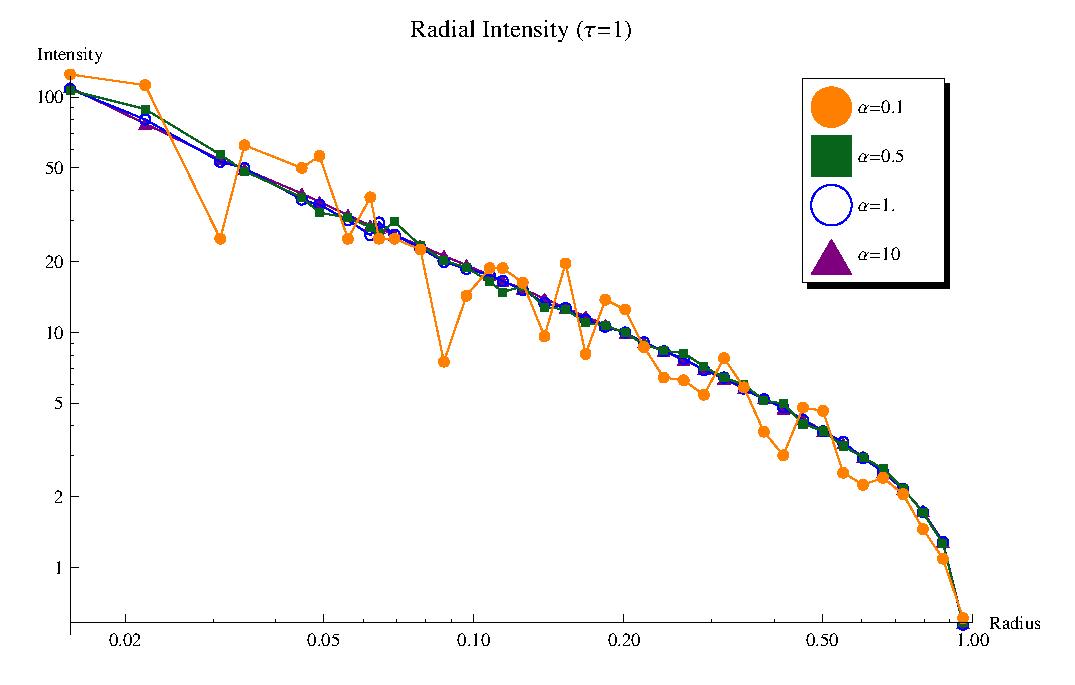
\includegraphics[width=1.0\textwidth]{mc3dalphasplot.eps}
			\caption{Bei gleicher Photonenzahl aber sinkendem Kamera--"Offnungswinkel $\alpha$ steigt der statistische Fehler aufgrund der geringeren Zahl beachteter Photnen.}
			\label{fig:alphacomparison}
		\end{figure}
	
	Die drei gew"ahlten optischen Tiefen $\tau\in\{0.01,1,10\}$ decken dabei den optisch d"unnen, mittleren und dicken Fall ab.	In Abb.~\ref{fig:methodcomparisongraphics} sind mit der analytischen Methode, \texttt{MC3D} und \texttt{PIRaTE} gewonnene radiale Intensit"atsprofile abgebildet.
	Im dargestellten Bereich stimmen die Ergebnisse beider Programme im Rahmen des statistischen Fehlers gut mit der analytischen L"osung "uberein. Dabei ist zu bedenken, da"s bei kleineren Radien "uber weniger Pixel der zugrundeliegenden Bilder gemittelt wird und somit der statistische Fehler dort naturgem"a"s gr"o"ser ausf"allt.
		\begin{figure}
			\centering
			\includegraphics[width=1.0\textwidth]{methodcomparisongraphics.eps}
			\caption{Vergleich zwischen der analytischen L"osung, \texttt{MC3D} und \texttt{PIRaTE} bei verschiedenen optischen Tiefen. \texttt{MC3D} hat f"ur alle drei F"alle $3.6\cdot10^8$ Photonen, \texttt{PIRaTE} jeweils $4.88\cdot10^7,4.88\cdot10^7,2.088\cdot10^8$ Photonenpfade generiert.}
			\label{fig:methodcomparisongraphics}
		\end{figure}
	\section{Einfaches Scheibenmodell}
	\subsection{Resultate}
	TODO: Vergleich mit MC3D (Ergebnis und Geschwindigkeit).
	Stichpunkte:tau=97.6958 in der Mittelebene. 1m55s f"ur $10^6$ Photonen mit MC3D. 720M Photonen in 72Ebenen $\rightarrow$ Jede Ebene entspricht 10M Photonen
	\section{Einordnung der Resultate}
	TODO: Gesamtvergleich zwischen MC3D und PIRaTE